
\clearpage
\section{Field Dynamics Applications}\label{manual:field-dynamics-applications}
\aodnoteblock{Scope}{This section uses the main-note field dynamics calculus as an application layer. SPARC uses the square-speed coordinate \(U=V^2\). The Tau ring fixture uses \(S_\tau\) and missing-burden diagnostics. Each score coordinate is declared inside its own support class.}

\aodremark{Field-dynamics simulations are finite compressions of the A\(\Omega\)D ontology. A macroscopic field is simulated by declared clustering, finite boundary windows, support families, and value maps. Output residuals are read against the declared data support: boundary placement, density resolution, time-flow data, angular/radial momentum inputs, slosh windows, capacity seating, and sheddic-route declarations.}

A large field-dynamics system is handled by declared clustering. A cluster records a retained family of distinctions and relations over a boundary/window. The cluster records its support expression, construction trace or inherited trace, capacity rule, coupling family, and route status. The cluster is a finite calculation container recording a declared A\(\Omega\)D form.



\subsection{Data-support classes for manual simulations and comparisons}\label{manual:field-dynamics-data-support-classes}
Dataset resolution selects the data-support class: radial rows instantiate G0; radial rows plus proxy density/current fields instantiate G1; three-dimensional density/velocity/current fields instantiate G2; time-ordered tracer positions/velocities instantiate G3. Each class reports residuals only in its declared coordinate. The table below records the manual classes used by this release.

\scriptsize
\begin{longtable}{@{}p{0.07\textwidth}p{0.17\textwidth}p{0.27\textwidth}p{0.22\textwidth}p{0.12\textwidth}@{}}
\caption{Data-support classes for manual simulations and comparisons.}\label{tab:manual-data-support-classes}\\
\toprule
Class & Name & Declared distinctions & Relations induced & Residual\\
\midrule
\endfirsthead
\toprule
Class & Name & Declared distinctions & Relations induced & Residual\\
\midrule
\endhead
D0 & exact internal fixture & exact integer gates, channels, comparator bins & internal returned-current relations & \(\delta_3\) tally\\
O0 & observable-map fixture & observable-map value and measured-sector target & external comparison map & target residual\\
G0 & radial shell projection & galaxy, radial bin, radius, speed, radial gas/disk/bulge support & radial shell field-dynamics relations & \(U\) residuals\\
G1 & radial-medium projection & G0 plus radial density/current proxy fields & radial medium-support relations & \(U\) + proxy\\
G2 & 3D shell field-dynamics retention & radial, angular, vertical cells; density, velocity, current, background support & local/inter/core/long/bg/J range SADAR & retention / field\\
G3 & time-resolved tracer-current simulation & G2 plus tracer positions/velocities through time windows & slosh, hinge shift, chiral flip, partial coupling & path / phase\\
L0 & exact lensing toy fixture & exact gates and comparator tallies & field-ring \(\delta_3\) relations & \(\delta_3\) tally\\
L1 & radial lens-medium diagnostic & radial medium proxies without image targets & medium-class relations & medium tallies\\
L2 & target-acquisition lane & image-count, Einstein-radius, image-position, or shear targets & target-side quarantine & acquisition\\
L3 & full lensing input package & declared medium fields, radiation-current gates, and target side & prediction before target join; target scoring after freeze & lens residuals\\
\bottomrule
\end{longtable}
\normalsize

\aodremark{This table records which distinctions are instantiated by a manual calculation. Projection and marginalization maps record comparison coordinates and uncertainty.}


\subsection{Data-support and uncertainty budget}\label{manual:field-dynamics-data-support-budget}
A field-dynamics diagnostic records its data-support and uncertainty budget before residuals are interpreted. The budget records the declared distinction family, support class, uncertainty component, and report target.

\scriptsize
\begin{longtable}{@{}p{0.16\textwidth}p{0.08\textwidth}p{0.42\textwidth}p{0.26\textwidth}@{}}
\caption{Field dynamics data-support classes.}\label{tab:field-dynamics-data-support-budget-a}\\
\toprule
Distinction family & Symbol & Declared data support & Support class\\
\midrule
\endfirsthead
\toprule
Distinction family & Symbol & Declared data support & Support class\\
\midrule
\endhead
Density & \(\epsilon_\rho\) & \(\rho(R,z,\theta,t)\) or radial proxy & 3D / 2D / radial / proxy\\
Velocity & \(\epsilon_v\) & \(v(R,z,\theta,t)\) or radial speed & vector / radial / proxy\\
Time window & \(\epsilon_\omega\) & cadence and duration & measured / declared / proxy\\
Boundary & \(\epsilon_{\partial}\) & \(\partial_T R_c(t)\) & 3D / radial / proxy\\
Capacity & \(\epsilon_C\) & \(C^{\mathrm{cap}}\) & typed / scalar / inherited / proxy\\
Coupling & \(\epsilon_E\) & \(E^{\mathfrak S}(B)\) & full / radial / proxy / ablation cut\\
Sheddic route & \(\epsilon_X\) & \(\operatorname{SheddicPath}\) & declared / inferred\\
External map & \(\epsilon_K\) & \(K_{\mathrm{ext}}\) or \(\lambda\) & frozen / calibrated\\
\bottomrule
\end{longtable}

\begin{longtable}{@{}p{0.16\textwidth}p{0.08\textwidth}p{0.32\textwidth}p{0.36\textwidth}@{}}
\caption{Field dynamics uncertainty and report targets.}\label{tab:field-dynamics-data-support-budget-b}\\
\toprule
Distinction family & Symbol & Uncertainty & Report target\\
\midrule
\endfirsthead
\toprule
Distinction family & Symbol & Uncertainty & Report target\\
\midrule
\endhead
Density & \(\epsilon_\rho\) & \(\sigma_\rho\) when declared & field or \(U\)\\
Velocity & \(\epsilon_v\) & \(\sigma_v\) & current, path, or \(U\)\\
Time window & \(\epsilon_\omega\) & \(\sigma_\omega\) & slosh / retention / path\\
Boundary & \(\epsilon_{\partial}\) & \(\sigma_{\partial}\) & boundary audits\\
Capacity & \(\epsilon_C\) & \(\sigma_C\) & retention / seating\\
Coupling & \(\epsilon_E\) & \(\sigma_E\) & retention / projection\\
Sheddic route & \(\epsilon_X\) & \(\sigma_X\) & route / slosh\\
External map & \(\epsilon_K\) & \(\sigma_{\mathrm{map}}\) & external comparison\\
\bottomrule
\end{longtable}
\normalsize

\aodremark{A scored diagnostic is interpreted within its declared support class. Projection and marginalization comparisons report their uncertainty records.}

\paragraph{Ablation cut.}
An ablation cut is a declared data-support cut with one distinction family intentionally omitted or marginalized. It records projection or marginalization residuals against a comparison support class. The evaluated A\(\Omega\)D form remains the declared form for that record.

\subsection{Scoped error forms by data-support class}\label{manual:field-dynamics-scoped-error-forms}
For a G0 radial shell projection, the score coordinate remains square speed:
\[
U^{\mathrm{obs}}_{g,j}=(V^{\mathrm{obs}}_{g,j})^2,
\qquad
\Delta U_{g,j}=U^{A\Omega}_{g,j}-U^{\mathrm{obs}}_{g,j}.
\]
If projection or input uncertainty is declared, the total uncertainty is recorded by
\[
\sigma^2_{\mathrm{total},g,j}
=
\sigma^2_{\mathrm{obs},g,j}
+
\sigma^2_{\mathrm{proj},g,j}
+
\sigma^2_{\mathrm{input},g,j},
\qquad
z^U_{g,j}=\frac{U^{A\Omega}_{g,j}-U^{\mathrm{obs}}_{g,j}}{\sigma_{\mathrm{total},g,j}}.
\]
For a G1 radial-medium projection, proxy-support residuals may be recorded as
\[
\epsilon_{\rho,j}=\rho^{A\Omega}_j-\rho^{\mathrm{proxy}}_j,
\qquad
\epsilon_{J,j}=J^{A\Omega}_j-J^{\mathrm{proxy}}_j.
\]
For a G2 three-dimensional field-dynamics retention fixture, exact retention tallies and field residuals may be recorded as
\[
\Delta^{\mathbb Z}_k=T_k-O_k,
\qquad
\delta_{3,k}=(s^{(3)}_k,m_k),
\]
\[
\epsilon_\rho(c)=\rho^{A\Omega}_c-\rho^{\mathrm{obs}}_c,
\qquad
J^{\mathrm{obs}}_c=\rho^{\mathrm{obs}}_c v^{\mathrm{obs}}_c,
\qquad
\epsilon_J(c)=J^{A\Omega}_c-J^{\mathrm{obs}}_c.
\]
When vector targets are declared, alignment may be recorded as
\[
\cos\alpha_c=\frac{J^{A\Omega}_c\cdot J^{\mathrm{obs}}_c}{\|J^{A\Omega}_c\|\,\|J^{\mathrm{obs}}_c\|+\varepsilon}.
\]
For a G3 time-resolved tracer-current fixture, path and velocity residuals such as \(\epsilon_x\) and \(\epsilon_v\) are declared against path-coordinate targets. RMSE reports are used only when the fixture declares metric units and path-coordinate targets.
\subsection{Two-dimensional slice / three-dimensional field toy}\label{manual:2d-3d-slice-toy}
This toy records how data-support scope changes the reported value when a three-dimensional field is represented by a two-dimensional slice or when the boundary is placed improperly. It is a manual diagnostic container that records declared comparison values.

Let \(B_{3D}\) be the declared three-dimensional boundary/window and let \(B_{2D}\) be the slice boundary obtained by suppressing the vertical/time-flow input. Let \(B_{\mathrm{bad}}\) be an intentionally improper setup boundary. The same calculation is evaluated three ways:
\[
U^{3D}_{\AO}=\mathsf Q^U_{\mathrm{ext}}(D^{\mathrm{BF}}(B_{3D})),
\qquad
U^{2D}_{\AO}=\mathsf Q^U_{\mathrm{ext}}(D^{\mathrm{BF}}(B_{2D})),
\qquad
U^{\mathrm{bad}}_{\AO}=\mathsf Q^U_{\mathrm{ext}}(D^{\mathrm{BF}}(B_{\mathrm{bad}})).
\]
The scoped diagnostics are
\[
\Delta U_{2D\to3D}=U^{2D}_{\AO}-U^{3D}_{\AO},
\qquad
\Delta U_{\partial}=U^{\mathrm{bad}}_{\AO}-U^{3D}_{\AO}.
\]
For exact internal bins, the same comparison may be recorded by
\[
\Delta_k^{\mathbb Z}=T_k^{\mathrm{bad}}-T_k^{3D},
\qquad
\delta_{3,k}(T^{\mathrm{bad}},T^{3D})=(s_k^{(3)},m_k).
\]

\small
\begin{longtable}{@{}p{0.18\textwidth}p{0.22\textwidth}p{0.24\textwidth}p{0.20\textwidth}@{}}
\caption{Toy data-support cases.}\label{tab:toy-data-support-cases}\\
\toprule
Case & Boundary / data & Diagnostic & Interpretation\\
\midrule
\endfirsthead
\toprule
Case & Boundary / data & Diagnostic & Interpretation\\
\midrule
\endhead
3D declared field & \(B_{3D}\), \(\rho(R,z,\theta,t)\), velocity and window data & baseline value \(U^{3D}_{\AO}\) or \(T^{3D}\) & retained support reference\\
2D slice & \(B_{2D}\), vertical/time-flow suppressed & \(\Delta U_{2D\to3D}\) & slice projection residual\\
Improper boundary & \(B_{\mathrm{bad}}\), wrong boundary/capacity/route & \(\Delta U_{\partial}\) or \(\delta_3(T^{\mathrm{bad}},T^{3D})\) & boundary-support residual\\
\bottomrule
\end{longtable}
\normalsize

\aodremark{This toy shows why field dynamics must record boundary declarations and data-support class. A two-dimensional slice and a three-dimensional field are different declared support classes; residuals between them are projection or boundary-support residuals before any external target comparison is interpreted.}



\subsection{3D Brownian phase-cycle \texorpdfstring{$\delta_3$}{delta3} fixture}\label{manual:brownian-phase-delta3-fixture}
\aodnoteblock{Data-support class}{This Brownian / tracer-motion fixture is a G3 time-resolved tracer-current fixture when the track declares time-ordered three-dimensional positions. A two-dimensional microscopy slice records its projection map or ablation cut.}

This fixture uses integerized three-dimensional trajectory data. A bacterium or tracer track is binned into \(\mathbb Z^3\); lagged displacements produce the active integer squared displacement
\[
Q_i^{(n)}=(a_i^{(n)})^2+(b_i^{(n)})^2+(c_i^{(n)})^2\in\mathbb Z_{\ge0}.
\]
Mass and size supply a candidate monon-beat scale \(\beta_a\). The trajectory is tested by displacement-bin counts, phase-cycle counts \(Q_i^{(n)}\bmod\beta_a\), octant direction counts, integer ratios, and exact \(\delta_3\) residuals. The full 3D coordinate phase-cycle specification is given in \appref{manual:app:coordinate-phase-cycle-delta3}.

The exact fixture path is
\[
z_i\in\mathbb Z^3\rightarrow\Delta z_i^{(n)}\rightarrow Q_i^{(n)}\rightarrow\theta_i^{(n)}\rightarrow O_\theta^{(n)}\rightarrow\delta_3.
\]
The retained trace path is
\[
\Delta z_i^{(n)}\rightarrow HT(h_i;B_{\mathrm{mot}})\rightarrow RD_{h_i}\rightarrow RCD_{h_i}\rightarrow\rho^D_{\omega,h_i}\rightarrow\SADARop_B.
\]


Continuous summaries belong after the exact fixture as presentation or external maps.

\aodnoteblock{Source artifacts}{The source package includes the Brownian application script under \texttt{manual/scripts} and the Brownian CSV rows under \texttt{manual/data/brownian}:
\[
\begin{gathered}
\texttt{aod\_brownian\_3d\_phase\_delta3.py},\quad
\texttt{displacement\_q\_counts.csv},\quad
\texttt{phase\_cycle\_delta3.csv},\\
\texttt{octant\_delta3.csv},\quad
\texttt{integer\_motion\_ratios.csv}.
\end{gathered}
\]
These Brownian application artifacts are aliases of the generic 3D coordinate phase-cycle fixture specified in \appref{manual:app:coordinate-phase-cycle-delta3}.}
\aodremark{Active coordinate: integerized three-dimensional displacement and phase-cycle count data,
\[
z_i\in\mathbb Z^3
\to \Delta z_i^{(n)}
\to Q_i^{(n)}
\to \theta_i^{(n)}
\to O_\theta^{(n)}
\to \delta_3.
\]
Continuous Brownian and diffusion-coefficient summaries are downstream presentation maps.}


\subsection{SPARC square-speed diagnostic}\label{manual:sparc-square-speed-diagnostic}
The SPARC five-galaxy square-speed score is the current G0 radial shell field-dynamics diagnostic lane. This record uses SPARC radial rotation-curve rows, scores the coordinate \(U=V^2\), forms \(\sigma_U=2V^{\mathrm{obs}}\sigma_V\) from the declared data uncertainty, and records \(\Delta U=U_{\AO}-U^{\mathrm{obs}}\) inside the G0 support class.
The SPARC benchmark supplies declared galaxy records
\[
\mathcal D_{\mathrm{SPARC}}
=\{G_i,r_{ij},V^{\mathrm{obs}}_{ij},\sigma_{V,ij},V^{\mathrm{gas}}_{ij},V^{\mathrm{disk}}_{ij},V^{\mathrm{bulge}}_{ij},\ldots\}.
\]
The score coordinate is square speed:
\[
U^{\mathrm{obs}}_{g,j}=(V^{\mathrm{obs}}_{g,j})^2,
\qquad
\sigma_{U,g,j}=2V^{\mathrm{obs}}_{g,j}\sigma_{V,g,j}.
\]
The uncertainty propagation is external benchmark arithmetic. The declared score target is \(U^{\mathrm{obs}}_{g,j}\), and benchmark input columns remain input data until the report map is evaluated.
\[
U^{\mathrm{bar}}_{g,j}
=
U^{\mathrm{gas}}_{g,j}
+
\Upsilon_d U^{\mathrm{disk}}_{g,j}
+
\Upsilon_b U^{\mathrm{bulge}}_{g,j}.
\]
The release constants are frozen before residuals are computed:
\[
\Upsilon_d=\frac12,
\qquad
\Upsilon_b=\frac{7}{10},
\qquad
K^U_{\mathrm{ext}}=8,
\qquad
J_{\mathrm{norm}}=1.
\]
The retained-window ratio uses the scalar duration accessor, not the RCD coupling object:
\[
\lambda^{\mathrm{ret}}_{g,j}:=\frac{\rho^D_{\omega,g,j}}{\rho^D_{g,j}}.
\]
The released field-dynamics support term is
\[
D^{\mathrm{BF}}_{g,j}
=
C_{\mathrm{cap},g,j}\lambda^{\mathrm{ret}}_{g,j}
\left(1+\frac{\mathrm{density}_{g,j}}{16}\right)
\left(1+\frac{\mathrm{gas/star}_{g,j}}{16}\right)
\left(1+\frac{\mathrm{bobbing}_{g,j}}{64}\right)J_{\mathrm{norm}}.
\]
In the five-galaxy G0/G1 diagnostic lane, the declared primary projection map uses
\[
C_{\mathrm{cap},g,j}=r_{g,j}
\left(|V^{\mathrm{gas}}_{g,j}|+|V^{\mathrm{disk}}_{g,j}|+|V^{\mathrm{bulge}}_{g,j}|\right),
\quad
\lambda^{\mathrm{ret}}_{g,j}=1,
\quad
\mathrm{density}_{g,j}=\mathrm{gas/star}_{g,j}=\mathrm{bobbing}_{g,j}=0.
\]
This neutral modifier convention belongs to the declared radial projection map. G1/G2/G3 packages carry angular, vertical, or time-flow fields through declared source or proxy rows.
The external square-speed map is
\[
U_{g,j,\AO}
=
U^{\mathrm{bar}}_{g,j}+K^U_{\mathrm{ext}}D^{\mathrm{BF}}_{g,j}.
\]
Here \(K^U_{\mathrm{ext}}\) is a quarantined external map coefficient frozen before scoring and used only by the external-comparison layer.
\[
\operatorname{scope}(K^U_{\mathrm{ext}})=\text{external square-speed value map},
\qquad
[K^U_{\mathrm{ext}}]=\frac{(\mathrm{km/s})^2}{\mathrm{kpc}\cdot(\mathrm{km/s})}=\frac{\mathrm{km/s}}{\mathrm{kpc}}.
\]
\aodliteraturenote{SPARC benchmark: SPARC database~\cite{sparc-database}, Lelli et al.~\cite{lelli-sparc-2016}.}
\aodnoteblock{Data-support class}{The SPARC five-galaxy lane instantiates a G0 radial shell data-support class. G0 active input fields are \(G_i,r_{ij},V^{\mathrm{obs}}_{ij},\sigma_{V,ij},V^{\mathrm{gas}}_{ij},V^{\mathrm{disk}}_{ij},V^{\mathrm{bulge}}_{ij}\). The report coordinate is \(U=(V^{\mathrm{obs}})^2\), \(\sigma_U=2V^{\mathrm{obs}}\sigma_V\), and \(\Delta U=U_{\AO}-U^{\mathrm{obs}}\). G1/G2/G3 packages carry angular, vertical, or time-flow fields through declared source or proxy rows.}

\subsection{SPARC five-galaxy scored records}\label{manual:sparc-five-galaxy-scored}
The five scored records are
\[
\{\mathrm{NGC2403},\mathrm{NGC3198},\mathrm{NGC6503},\mathrm{NGC2841},\mathrm{DDO154}\}.
\]
Data files, scored outputs, and the regeneration script are included in the source package:
\[
\begin{aligned}
&\texttt{manual/data/sparc},\\
&\texttt{manual/data/derived/sparc\_five\_galaxy\_per\_bin.csv},\\
&\texttt{manual/data/derived/sparc\_five\_galaxy\_per\_galaxy.csv},\\
&\texttt{manual/scripts/score\_sparc\_field\_dynamics.py}.
\end{aligned}
\]
\aodremark{The SPARC five-galaxy scored records are generated from the included rotation-curve files and the frozen declaration constants listed in this section.}
\[
\Delta U_{g,j}=U_{g,j,\AO}-U^{\mathrm{obs}}_{g,j},
\qquad
z^U_{g,j}=\frac{\Delta U_{g,j}}{\sigma_{U,g,j}}.
\]
\[
\chi^2_{U,g}=\sum_j(z^U_{g,j})^2,
\quad
MAE_{U,g}=\frac{1}{N_g}\sum_j|\Delta U_{g,j}|,
\quad
MSE_{U,g}=\frac{1}{N_g}\sum_j(\Delta U_{g,j})^2.
\]
\[
MAPE_{U,g}=\frac{100}{N_g}\sum_j\left|\frac{\Delta U_{g,j}}{U^{\mathrm{obs}}_{g,j}}\right|,
\qquad
U^{\mathrm{obs}}_{g,j}>0.
\]
Bins are excluded only by a predeclared data-quality rule or by a predeclared denominator floor.
\begin{table}[H]
\centering
\scriptsize
\caption{SPARC five-galaxy scored records. Data-support class is G0 for this radial shell projection lane; the uncertainty policy is observation-only in this release.}
\begin{tabular}{lccrrrrr}
\toprule
$G$ & Class & $\sigma$ policy & $N$ & $\chi^2_U$ & $MAE_U$ & $MSE_U$ & $MAPE_U$ [\%]\\
\midrule
DDO154 & G0 & obs-only & 12 & 10893.83 & 697.2 & 602049.7 & 41.42\\
NGC2403 & G0 & obs-only & 73 & 22038.64 & 2486.2 & 7212253.2 & 23.31\\
NGC2841 & G0 & obs-only & 50 & 3235.74 & 23910.7 & 674670051.2 & 26.47\\
NGC3198 & G0 & obs-only & 43 & 6352.96 & 5478.2 & 62935093.1 & 37.51\\
NGC6503 & G0 & obs-only & 31 & 718.93 & 1697.4 & 3689898.7 & 13.50\\
\bottomrule
\end{tabular}
\label{tab:manual-sparc-five-galaxy-scores}
\end{table}

\begin{figure}[H]
\centering
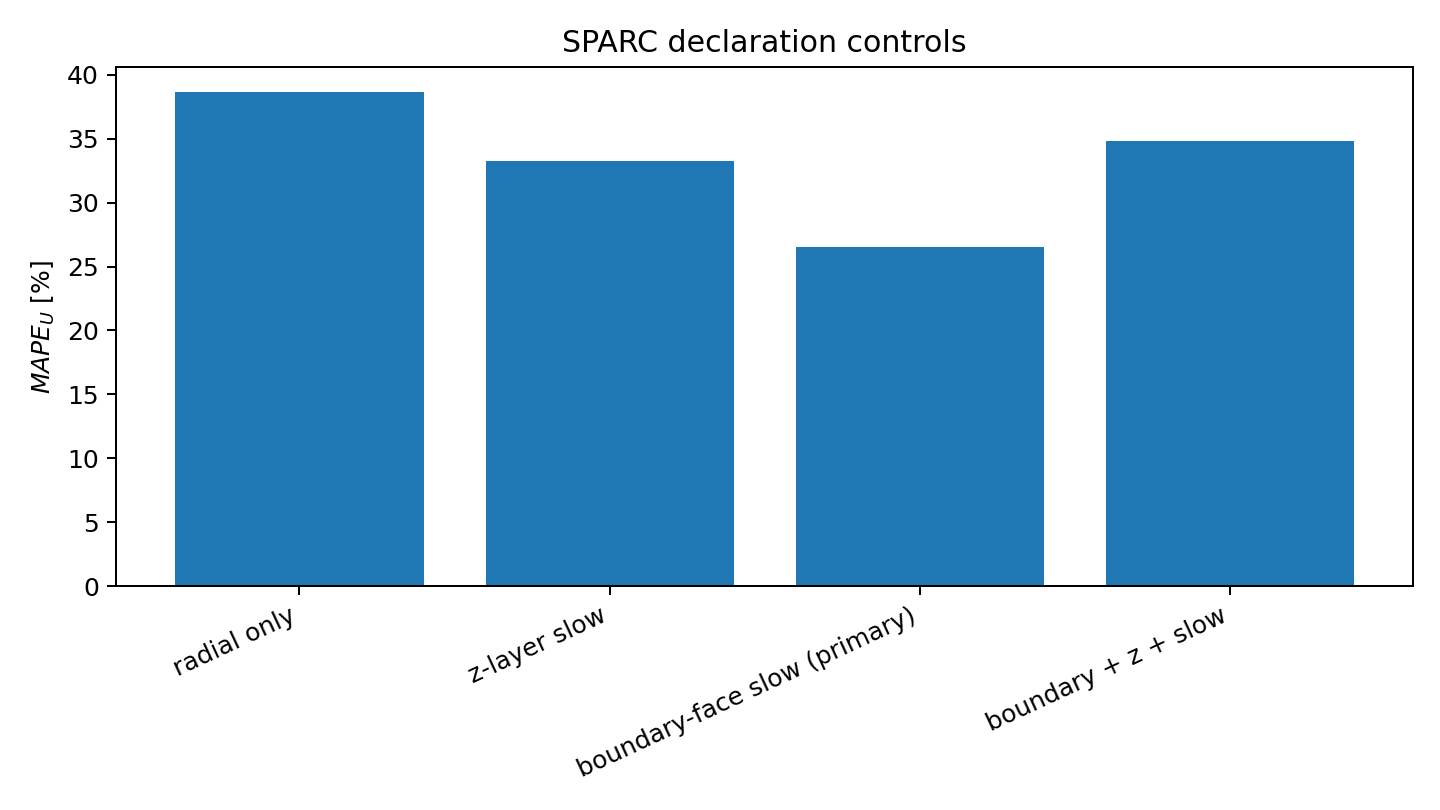
\includegraphics[width=0.82\linewidth]{figures/sparc_declaration_controls.png}
\caption{SPARC declaration controls. The score is \(MAPE_U\) across the five-galaxy benchmark sample.}
\label{fig:manual-sparc-controls}
\end{figure}
\begin{figure}[H]
\centering
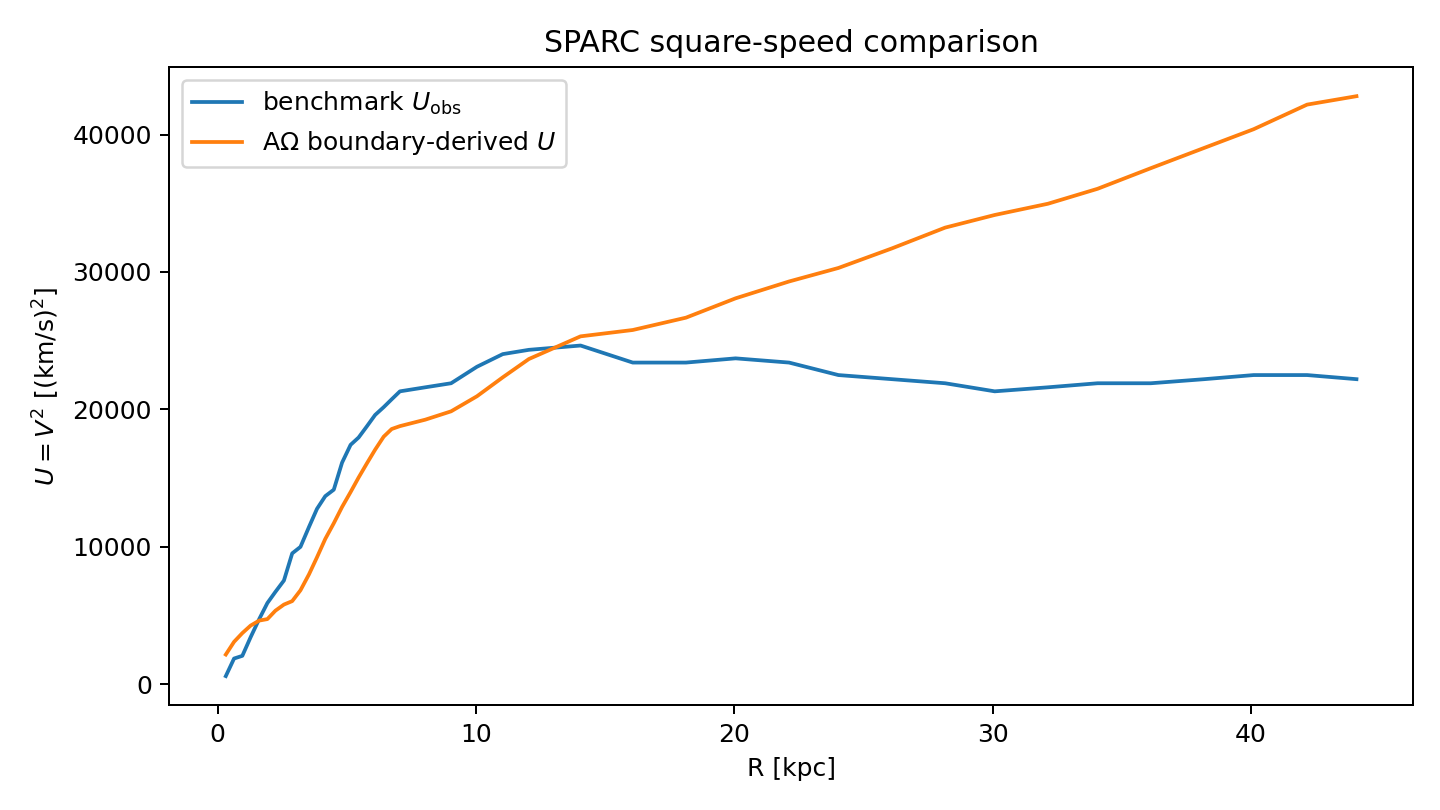
\includegraphics[width=0.82\linewidth]{figures/sparc_square_speed_comparison.png}
\caption{SPARC square-speed comparison for the NGC3198 display record. The scored coordinate is \(U=V^2\).}
\label{fig:manual-sparc-square-speed-comparison}
\end{figure}
\begin{figure}[H]
\centering
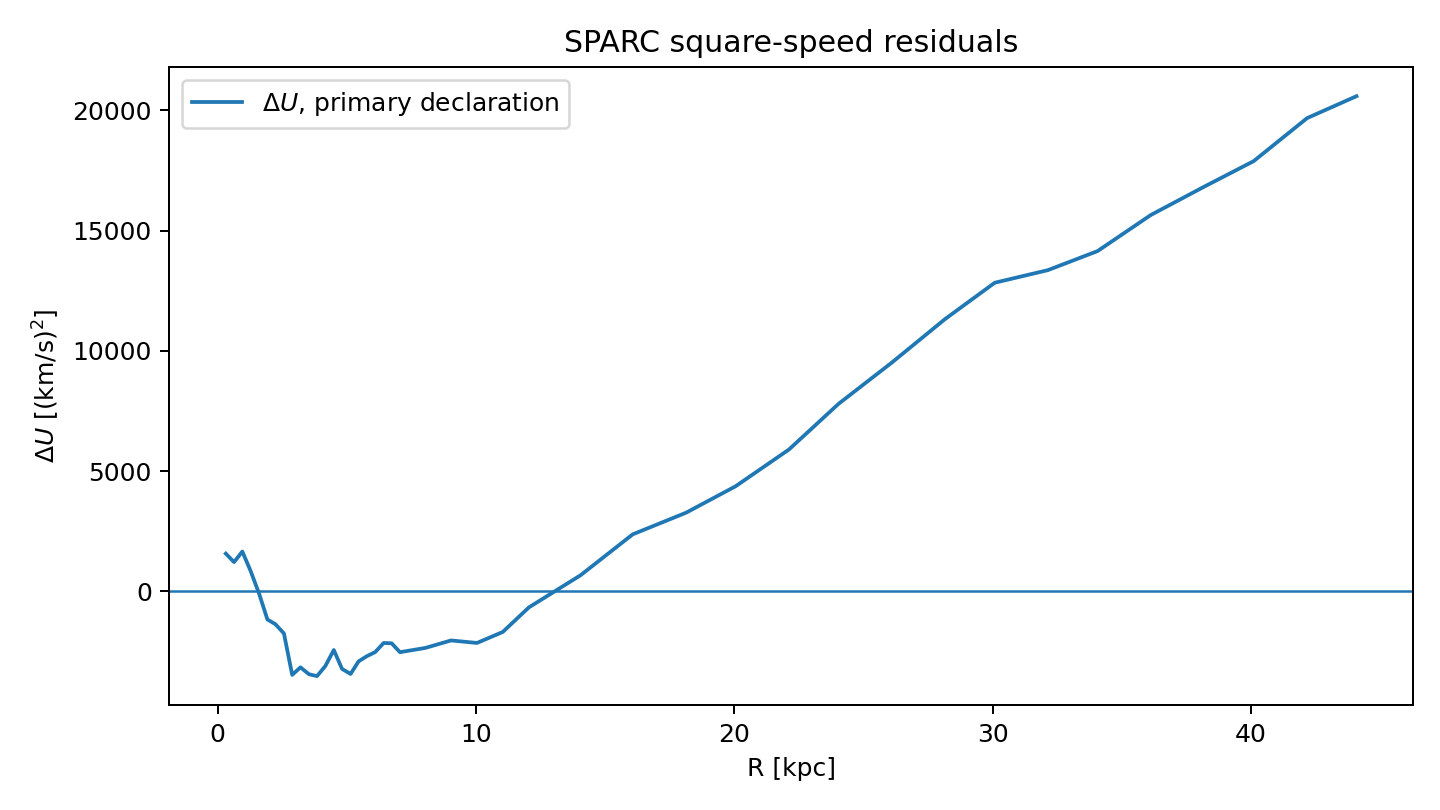
\includegraphics[width=0.82\linewidth]{figures/sparc_square_speed_residuals.png}
\caption{SPARC square-speed residuals for the NGC3198 display record. The residual is \(\Delta U=U_{\AO}-U_{\mathrm{obs}}\).}
\label{fig:manual-sparc-residuals}
\end{figure}
\begin{figure}[H]
\centering
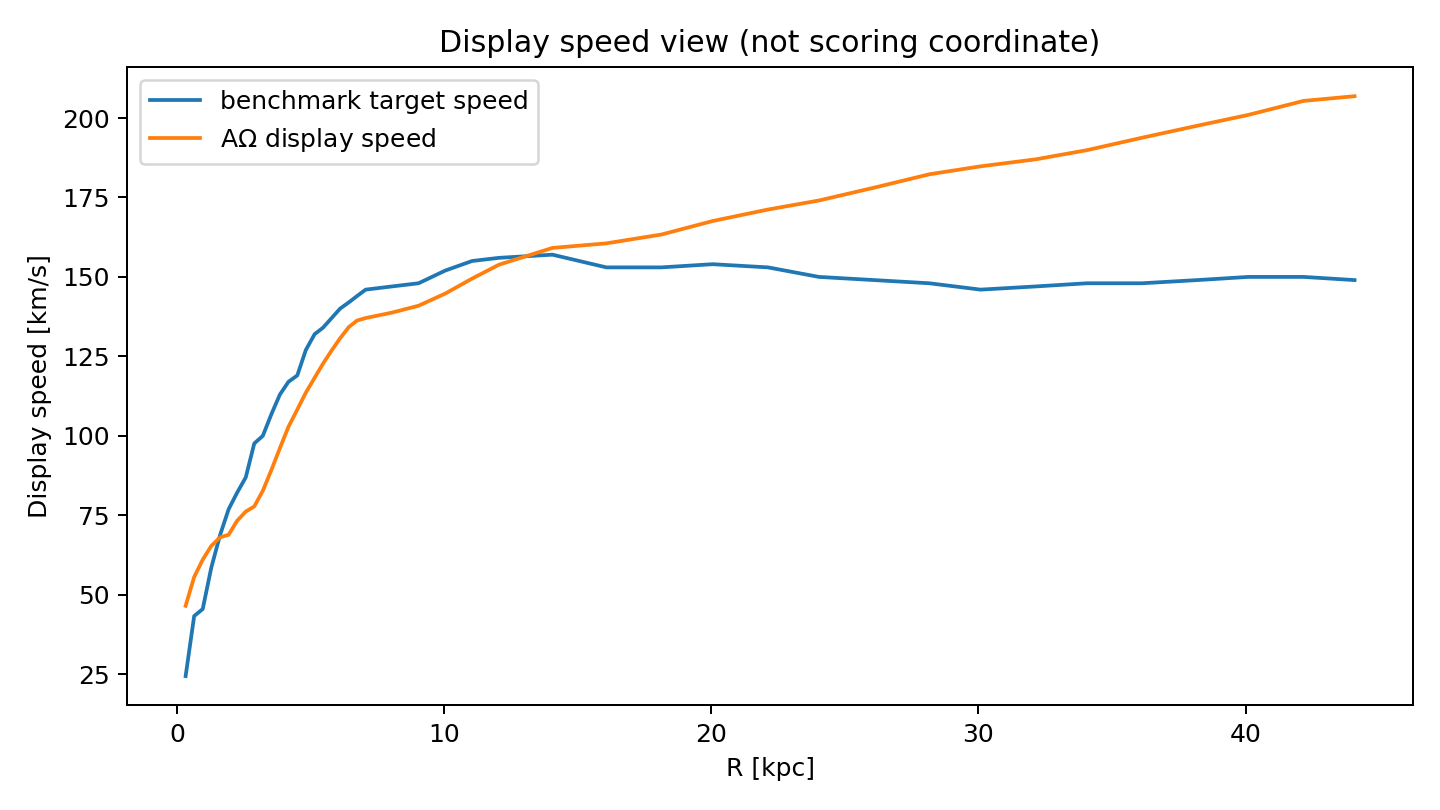
\includegraphics[width=0.82\linewidth]{figures/sparc_display_speed_view.png}
\caption{Display speed view. This presentation view uses \(V_{\mathrm{disp}}=\sqrt U\) after scoring; the score coordinate is \(U\).}
\label{fig:manual-sparc-display-speed}
\end{figure}

\subsection{Tau ring diagnostic fixture}\label{manual:tau-ring-diagnostic}
The Tau ring fixture uses \(S_\tau\), \(S_{\tau,\mathrm{ring}}\), missing fraction, and winner margin.
\[
\mathcal K_\tau=\{1{:}2{:}8,1{:}2{:}9_{\mathrm{yro}},1{:}2{:}10,3{:}3{:}8\}.
\]
\[
K_\tau^\star=\arg\min_{K\in\mathcal K_\tau}|S_{\tau,\mathrm{ring}}(K)|.
\]
The rerun selects
\[
\boxed{K_\tau^\star=1{:}2{:}9_{\mathrm{yro}}=\mathrm{Dimonnanyro}.}
\]
For the primary lane,
\[
1{:}2{:}9:
\qquad
S_\tau=-0.036807,
\qquad
S_{\tau,\mathrm{ring}}=-0.105804.
\]
The missing-burden diagnostic records the exact ratio
\[
\mathrm{miss}_\tau(1{:}2{:}9_{\mathrm{yro}})=\frac{31}{50},
\qquad
\mathrm{missing\_fraction\_display}=0.62.
\]
\aodnoteblock{Precision note}{Support identities and candidate declarations are exact. Plotted scores are diagnostic presentation decimals from the analysis script and are not A\(\Omega\) primitives.}
\begin{figure}[H]
\centering
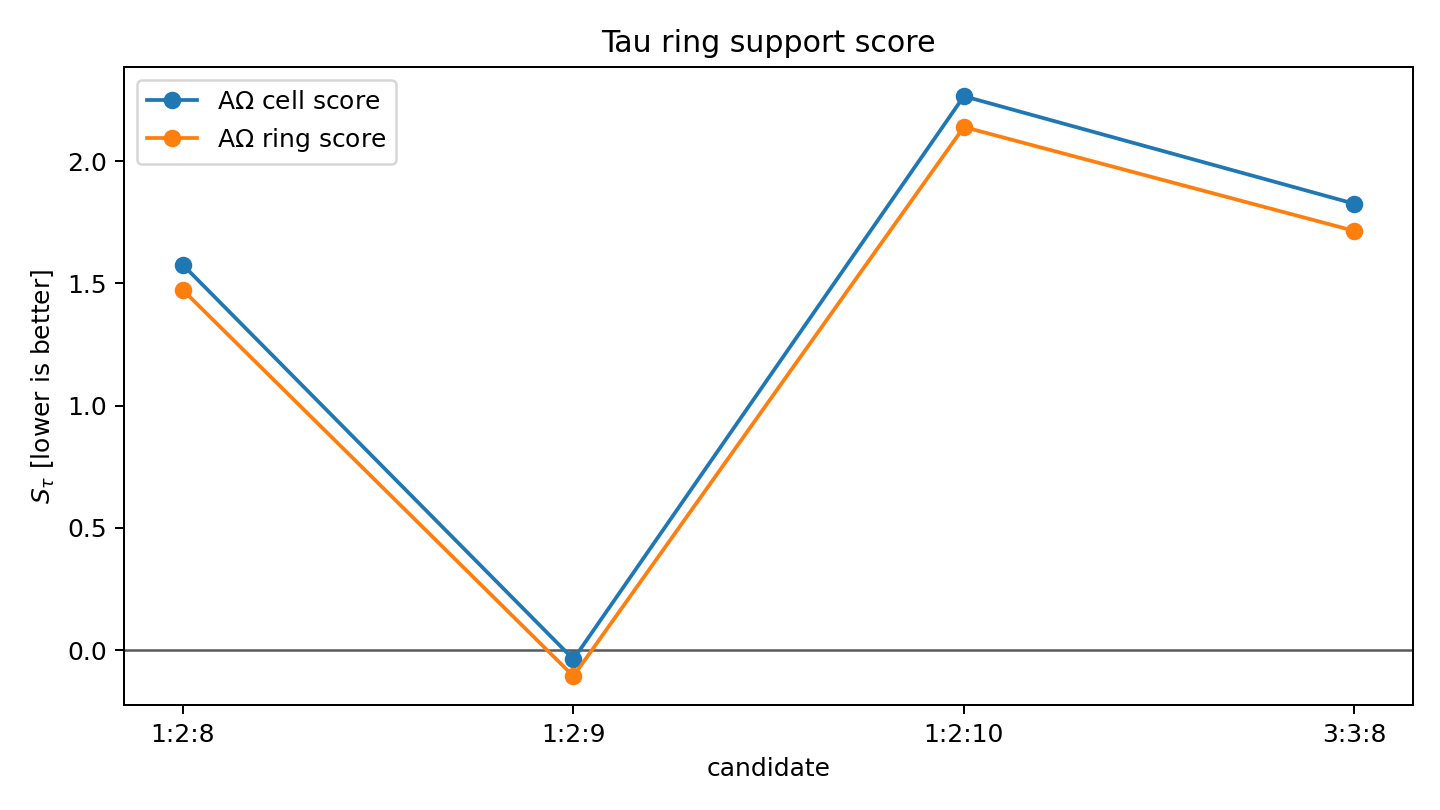
\includegraphics[width=0.82\linewidth]{figures/tau_ring_support_score.png}
\caption{Tau ring support score. The ring diagnostic preserves \(1{:}2{:}9_{\mathrm{yro}}\) / Dimonnanyro as the closest candidate.}
\label{fig:manual-tau-ring-score}
\end{figure}
\begin{figure}[H]
\centering
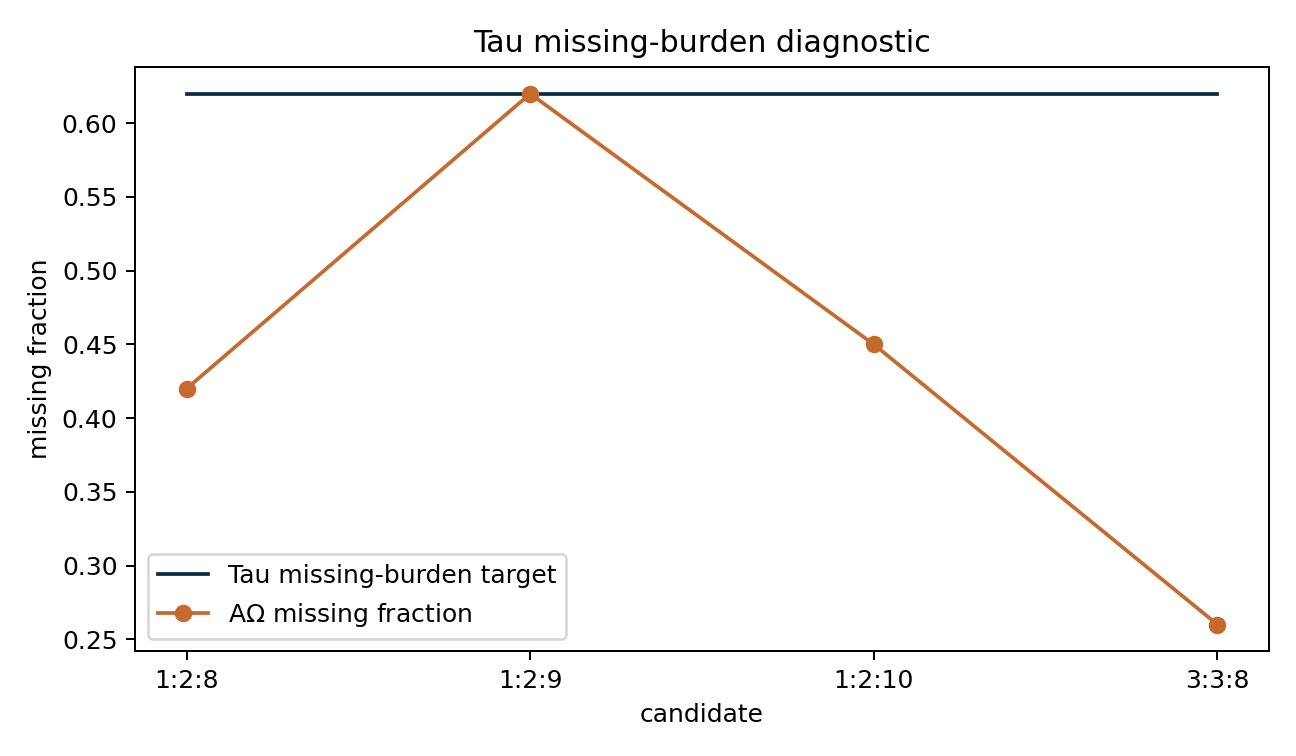
\includegraphics[width=0.82\linewidth]{figures/tau_missing_burden_diagnostic.png}
\caption{Tau missing-burden diagnostic. The plot renders the exact missing-burden ratio \(31/50\) as the presentation value \(0.62\) for the \(1{:}2{:}9_{\mathrm{yro}}\) / Dimonnanyro row.}
\label{fig:manual-tau-missing}
\end{figure}
\begin{figure}[H]
\centering
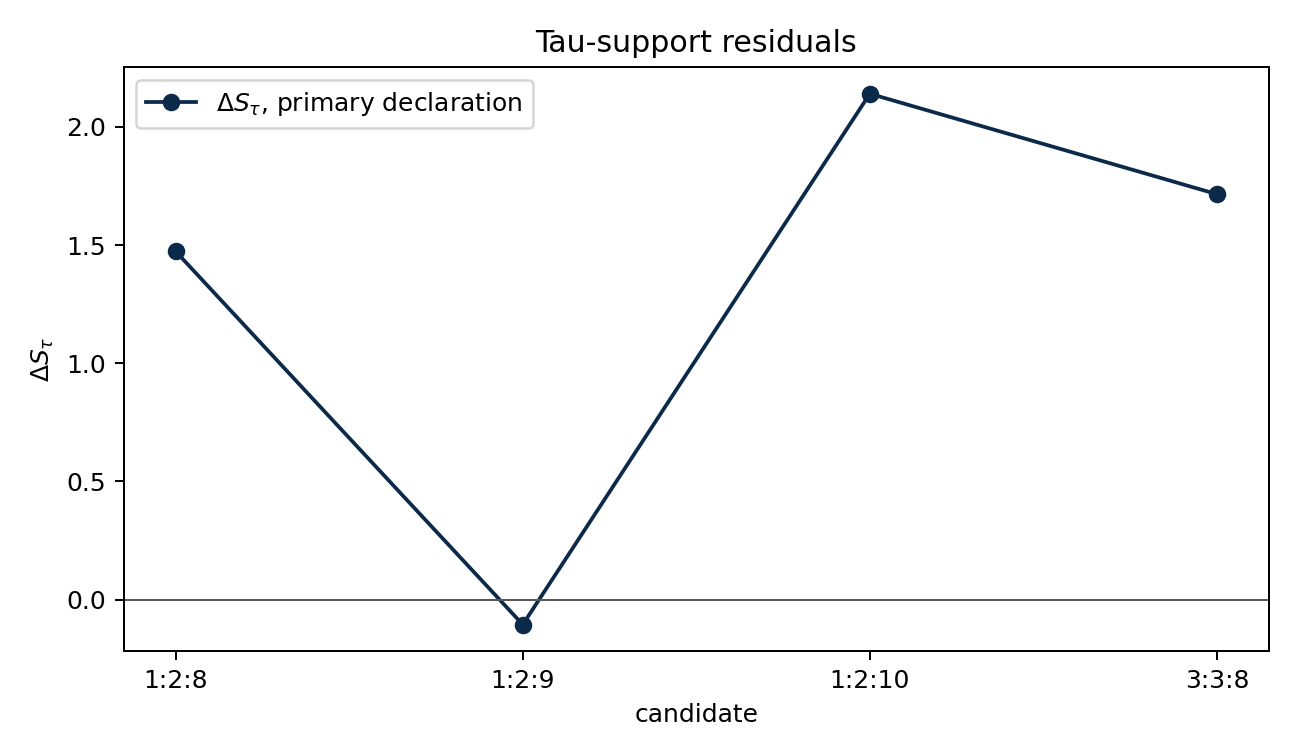
\includegraphics[width=0.82\linewidth]{figures/tau_support_residuals.png}
\caption{Tau-support residuals against the declared support-score target.}
\label{fig:manual-tau-residuals}
\end{figure}
\begin{figure}[H]
\centering
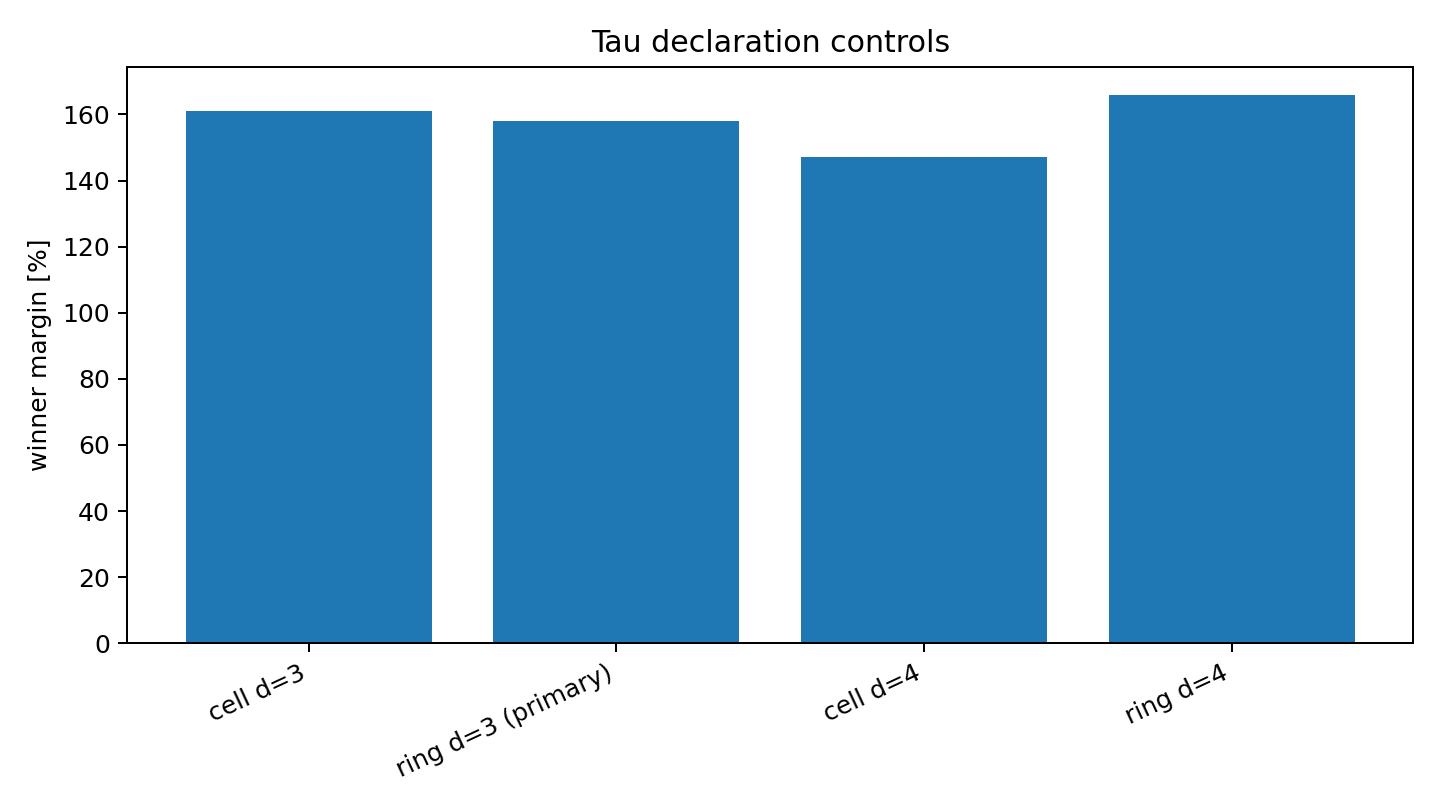
\includegraphics[width=0.82\linewidth]{figures/tau_declaration_controls.png}
\caption{Tau declaration controls. Labels are declaration controls for the internal diagnostic lane.}
\label{fig:manual-tau-controls}
\end{figure}

\subsection{Milky Way / Gaia follow-up declaration}\label{manual:mw-gaia-followup}
The Sol bobbing record is recorded as a field dynamics diagnostic.
\[
B_{\mathrm{Sol}}|t=(\partial_T R_{\mathrm{Sol}}(t),\omega_{\mathrm{Sol}}|t).
\]
\[
\Phi^D_{\partial_T R,\mathrm{mov}}(t)
=\Phi^D_{\mathrm{cross}}(t)-\Phi^D_{\mathrm{sweep}}(t)+\Phi^D_{\mathrm{shedding}}(t).
\]
A Gaia follow-up comparison is recorded after a benchmark target record is supplied.


\subsection{Orbital-retention field-dynamics fixture plan}\label{manual:orbital-retention-field-dynamics-fixture}
Data-support class: G2/G3 retention-first field-dynamics fixture. Its sequence is
\[
\begin{aligned}
&\text{medium setup}\rightarrow\text{flip/fizz classification}\rightarrow\text{range-prioritized SADAR},\\
&\text{capacity seating}\rightarrow\text{orbital retention}\rightarrow\text{\(\delta_3\) class tally},\\
&\text{optional }U\text{ diagnostic}.
\end{aligned}
\]
The fixture declares the flip classifier inside the manual/application layer:
\[
\operatorname{FlipClass}_{e,c,t}
\in
\{\mathrm{early\_coupling},\mathrm{fizz},\mathrm{pending},\mathrm{sheddic\_route}\}.
\]
The early-coupling indicator is
\[
G^{\mathrm{early}}_{e,c,t}
=
\mathbf 1[\rho^D_{\omega,e,c,t}>0]\,
\mathbf 1[Q^D_{e,c,t}<Q_{\max}]\,
C^{\theta}_{e,c,t}\,
Z^{\mathrm{imp}}_{e,c,t}\,
\mathbf 1[\Delta A_{e,c,t}\ne0].
\]
When \(G^{\mathrm{early}}_{e,c,t}>0\), the fixture records early coupling. Fizz records successor motion / background-continuation jitter. Pending records retained return carried over the current window. The class \(\mathrm{sheddic\_route}\) records a flip carried through a declared sheddic path.


\paragraph{Orbital-retention input provenance gate.}
Before a scored orbital-retention run, the fixture records the data provenance of every field component used by the retained calculation. The input package records radial support rows; three-dimensional density fields; gas/stellar velocity fields; momentum fields; time-window/slosh fields; capacity rule; coupling family; sheddic-route declaration; and external value map when used. SPARC radial rows may populate the radial-support component. Three-dimensional density, velocity, current, and time-flow components are populated by their own declared source rows or proxy rows before scoring.

\scriptsize
\begin{longtable}{p{0.19\textwidth}p{0.17\textwidth}p{0.17\textwidth}p{0.20\textwidth}p{0.09\textwidth}}
\caption{Orbital-retention input provenance gate.}\label{tab:orbital-retention-input-provenance}\\
\toprule
Field component & Source & Support status & Uncertainty status & Scored\\
\midrule
\endfirsthead
\toprule
Field component & Source & Support status & Uncertainty status & Scored\\
\midrule
\endhead
stellar radial support & SPARC radial model & SPARC-supported radial & radial source row & diagnostic\\
stars, full medium & 3D stellar density & external 3D & measured / proxy & if declared\\
gas, full medium & H I / H\(\alpha\) / IFU field & external 3D & channel / velocity uncertainty & yes, if declared\\
core / background & model or survey & latent / proxy & proxy recorded & conditional\\
current-cycle family & A\(\Omega\)D range edges & declared proxy & declaration audit & internal\\
time-flow / slosh & kinematic window & external 3D / latent & cadence / window & conditional\\
external value map & quarantined map & declared proxy & frozen before scoring & external only\\
\bottomrule
\end{longtable}
\normalsize

\aodremark{A scored orbital-retention run records source, support status, uncertainty status, and whether each component is used for scoring before residuals are interpreted.}

\small
\begin{longtable}{@{}p{0.08\textwidth}p{0.34\textwidth}p{0.42\textwidth}@{}}
\caption{Orbital-retention field-dynamics fixture spine.}\label{tab:orbital-retention-fixture-spine}\\
\toprule
No. & Sheet & Purpose\\
\midrule
\endfirsthead
\toprule
No. & Sheet & Purpose\\
\midrule
\endhead
00 & Declarations & Freeze declarations before scoring.\\
01 & Cell grid 3D & Declare the retained 3D cell grid.\\
02 & Input density fields & Declare star/gas/core/background/current density inputs and source/status records.\\
03 & Fractal range / max field support & Compute fractal range and maximum supported field count.\\
04 & Field regime & Declare gas/fluid/fizz regime.\\
05 & Chiral flip: early coupling vs fizz & Classify flips as early coupling, fizz, pending, or sheddic route.\\
06 & Range edge sets & Build range-prioritized coupling families.\\
07 & SADAR coupling / pressure / velocity & Compute SADAR coupling, pressure, and motion quantities.\\
08 & Capacity seating & Seat capacity by range and closure state.\\
09 & Hinge shift / partial coupling & Record hinge shift and partial coupling.\\
10 & Slosh / sheddic / pending & Record slosh, sheddic routing, and pending return.\\
11 & Orbital retention class & Classify orbital retention before projection.\\
12 & Delta3 retention tallies & Record exact \(\delta_3\) retention tallies.\\
13 & U projection diagnostic & Optional square-speed diagnostic after retention scoring.\\
14 & Audit & Check declaration, retention, projection, and error layers.\\
\bottomrule
\end{longtable}
\normalsize

\aodremark{The SPARC square-speed lane is a G0 radial projection diagnostic. The orbital-retention fixture is the G2/G3 retention-first simulation path. Projection to \(U\) follows retention, capacity seating, and \(\delta_3\) tallies.}

\subsection{Completion requirements}\label{manual:field-dynamics-completion-requirements}
A SPARC scored record is complete when the data file, declaration constants, square-speed target, residuals, and score metrics are present. A Tau ring fixture is complete when the candidate set, scores, missing fraction, and precision note are present. Display speed is a presentation view only. The orbital-retention field-dynamics fixture is complete when it records medium setup, flip/fizz classification, range-prioritized SADAR, capacity seating, retention class, and \(\delta_3\) tallies.
